\section{Small scale auroral features and Alfvén waves}
Starting in the 1950s and 1960s, auroral morphology from the polar regions and auroral oval down to the mid latitudes \citep{akasofu1963} was rigorously studied.
The discovery of the magnetosphere and early understanding of its processes and regions by the mid-1960s hastened the instrument development cycle, both space- and ground-based.
Descriptions of auroral morphology depend strongly on the viewing perspective due to~\eqref{eq:bint}.
The viewer directly beneath the aurora of Figure~\ref{fig:chernouss6}(a) sees ribbons of aurora while the viewer roughly \unit[100]{km} away sees auroral curtains in Figure~\ref{fig:chernouss6}(b)--despite looking at the same section of aurora.
To motivate the disentangling of this difficult observational problem in chapter~\ref{chapter:sim}, a discussion of the processes driving microscale aurora is in order.

Despite the highly complex and time-varying linkages and paucity of coördinated \textit{in situ} measurements, a first step in understanding a ``black box'' system is quantifying the energy flux for the system and its components.
Cold ionospheric plasma, mirroring particles, the plasma sheet and direct injection from the solar wind are among  ultimate sources of precipitating particles driving the aurora.
Particle momentum carries particles across the solar system, with shocks and pickup ions redirecting the guiding center trajectory.
The structure of structured aurora is oriented along the $B_\perp$ dimension due to the frozen-in condition of plasma causing the guiding center of particles to follow geomagnetic field lines.
Structured aurora is a projection of acceleration structures in the 3000..\unit[10000]{km} altitude range.
When discussing the atmosphere, ionosphere and magnetosphere, altitude is given above mean sea level.
The finest ground-observable structures are of order \unit[10..100]{m} from even filamental electron beams due to diffusion in the ionospheric column traversed \citep{borovsky1993}.

Throughout this dissertation, ``ion'' is synonymous with a particle of positive charge. Some of the important species in the ionosphere include N$_2$, O, and N$_2^+$. 
While solar radiation throughout the ultraviolet (UV) range is responsible \citep{rees1989} for creating much of the plasma in the ionosphere, accelerated electrons are the primary driver of the aurora. 
Assumptions used in the analysis include:
\begin{enumerate}
    \item Precipitating electron energies $E > \unit[100]{eV}$
    \item Average energy loss per ionization is \unit[35.5]{eV}
    \item Excitation requires energy \unit[1..100]{eV}
%    \item \citep{semeter2005} %paragraph 17
\end{enumerate}
``Cold'' ionospheric plasma has energies of a few eV, much less than the 35~eV needed to emit a photon.
Solar wind particles have energies of order \unit[100]{eV} \citep{mottez2015}.
Only about 1\% of the $1.3 \times 10^{13}$~W flux intercepting Earth's magnetosphere is captured into the magnetosphere system \citep{mottez2015}.
Most of the intercepted flux is stored in the magnetotail, which explosively discharges every several hours in substorms, taking a few hours to restore the magnetosphere to a relaxed state, which is already recharging with solar wind flux for the next cycle.
The shear forces and turbulence in general associated with reconfiguration in any magnetic system must be communicated to other portions of the magnetoplasma.
Alfvén waves are a key mechanism for releasing stress in dynamic magnetoplasma systems.

\FloatBarrier
\subsection{Alfvén Waves}\label{sec:alfven}
Plasmas infused with magnetic field $B$ are subject to perturbations that send energy across vast distances.
On intergalactic scales, Alfvén waves have been thought to have a possible role in the evolution of cosmic rays \citep{matsukiyo2009}.
In the solar wind, theory and modeling have shown a possible role in instabilities leading to filamentation of Alfvén waves and corresponding perturbations in plasma density and $B$ \citep{kuo1988}.
In the geomagnetic system, stresses and reconfigurations from geomagnetic storms and substorms are communicated with speeds reaching to order $0.1c$. 
Alfvén waves communicate information about the constantly reconfiguring geomagnetic system across scales and great distances.

In general Alfvén waves may propagate obliquely to $B$, but for observable outcomes of electron acceleration by Alfvén waves, we assume that the Alfvén wave electric field is oriented approximately parallel to $B$.
The fingerprints of Alfvénic aurora due to Alfvén wave electron acceleration may be seen in measurements back at least to the 1970s.
The theory and modeling were solidified in the 2000s by works such as \citet{stasiewicz2000,chaston2003,chaston2007how}.
Although large fluxes of Alfvén wave-accelerated electrons in the \unit[1..10000]{eV} range are responsible for many dramatic structured auroral displays \citep{chaston2003}, numerous other methods of auroral acceleration exist \citep{borovsky1993}.

Waves in media may have fields oriented longitudinally, transverse, or oblique to the direction of propagation $\hat{k}$. 
Longitudinal waves are also known as \textit{compression} waves and transverse waves are also known as \textit{shear} waves.
Alfvén waves can reflect off the ionosphere and plasma sheet in the magnetotail repeatedly. 
Instabilities generated in ionospheric plasma by Alfvén waves have been shown by observation and modeling to be a plausible candidate for ion upflow \citep{chaston2004}, without directly involving heating \citep{zett2007,zett2008}.
Subsets of IAW such as solitary IAW and dissipative nonlinear IAW have been proposed as consistent with narrow auroral features \citep{wu2004}.
Alfvén waves have been shown to be a primary driver of dynamic aurora via \textit{in situ} observations including DMSP and FAST measurements compiled over several years.
As recounted in \citet{stasiewicz2000}, Hannes Alfvén's development and the observational confirmation of Alfvén wave theory parallels that of J. C. Maxwell's elucidation of electromagnetism.
Distinguishing between intra-Alfvénic and non-Alfvénic wave electron acceleration, essential to the $B_\perp$ structure of kinetic plasma behavior, is enhanced by the equipment described in chapter~\ref{chapter:inst} and analysis in chapters~\ref{chapter:sim} and~\ref{chapter:fusion}.

The electron thermal velocity is
\begin{equation}
v_{te} = \sqrt{2\frac{T_e}{m_e}}
\end{equation}
while Alfvén waves propagate with Alfvén velocity
\begin{equation}
v_A = \frac{B_0}{\sqrt{\mu_0\rho}}
\end{equation}
and Alfvén wave frequency
\begin{equation}
\omega = k_\parallel v_A
\end{equation}
where $v_A \ll c$ in many geomagnetic plasmas, $T_e$ is electron temperature, $m_e$ is the electron mass, $\rho=n_im_i$ is the mass density, $B_0$ is the local geomagnetic field strength and $\mu_0$ is the vacuum permeability \citep{stasiewicz2000}.
As $v_A \Rightarrow c$, the Alfvén wave behaves increasingly as if in a non-magnetized medium.
The rules of phase reversal upon reflection are the same for Alfvén waves as for general TEM waves.
Two Alfvén wave regimes referred to collectively as dispersive Alfvén waves (DAW) are described in Table~\ref{tab:alfven} and section~\ref{sec:alfvenaccel}.
\begin{table}\centering
	\caption{Dispersive Alfvén wave types relevant to auroral acceleration \citep{stasiewicz2000}.}
    \label{tab:alfven}
	\begin{tabular}{ccccc}
        \toprule
		Alfvén wave type & frequency & speed & pressure & altitude [km] \\
		\midrule
		inertial & $\omega < \omega_{ci}$  & $v_A > v_{te} $  & $ \beta < \frac{m_e}{m_i} $ & 3,000..20,000 \\ % Staciewicz 2001 pg. 429
		kinetic & & $v_A < v_{te}$ & $\frac{m_e}{m_i} < \beta < 1$ & $\gtrsim 20,000$ \\
        \bottomrule
	\end{tabular}
\end{table}


\FloatBarrier
\subsection{Alfvénic Auroral Acceleration}\label{sec:alfvenaccel}
Electron-driven aurora can most broadly be categorized as diffuse or discrete \citep{newell2009}.
Diffuse and structured auroral arcs driven by inverted-V potential structures may be time-modulated in flux by ion-acoustic resonances.
Regions with sharp potential gradients are included in the category of inverted-V precipitation driven aurora, along with the smoothly varying potential structure the name implies \citep{newell2009}.
Inverted-V arcs may translate, but they do not experience splitting or flaming behavior, and NEIALs are not associated with them.
The diffuse aurora life cycle is dominated by resonant wave-particle interactions scattering plasma sheet electrons in the loss cone \citep{Ni2016}.
Time-modulated diffuse aurora is driven by mechanisms with little dispersion relative to discrete auroral drivers.
\begin{figure}\centering
	\begin{tikzpicture}
	\node (mirror) [startstop] {Mirroring ions and electrons \par };
	
	\node (fac) [process,below of=mirror,xshift=-3cm,yshift=-0.5cm] {FAC \par};
	
	\node (ion) [startstop,below of = fac,text width=3cm,yshift=-0.5cm] {ion/electron diffuse aurora \par};
	
	\node (inv) [process,right of = fac,xshift=4cm] { Inverted-V, double layer \par};
	
	\node (mono) [startstop,below of = inv,text width=4cm,yshift=-0.5cm] { Discrete, monoenergetic aurora \par };
	
	
	\draw[arrow] (mirror) -- (fac);
	\draw[arrow] (fac) -- (ion);
	
	\draw[arrow] (mirror) -- (inv);
	\draw[arrow] (inv) -- (mono);
	
	\end{tikzpicture}
	\caption{Block diagram of non-Alfvénic aurora acceleration mechanism.}
	\label{fig:nonalfvenblock}
\end{figure}

\citet{chaston2007how,mcfadden1999} note that particle acceleration relevant to ground-observable aurora occurs along $B_\parallel$ and occurs in altitude ranges from about 3000..\unit[20000]{km}.
\citet{stasiewicz2000} cited Freja measurements showing that while cold plasma $\sim \unit[5]{eV}$ heavily dominates from 1000..8000~km in the auroral zone and polar cap, in Alfvénic turbulence regions almost no cold electrons exist.
The source of sudden large flux of low energy electrons is thought to come from Alfvén wave acceleration of mirroring electrons into the loss cone.
Alfvén waves operate across a wide range of regimes from accelerating relativistic particles in galaxy clusters \citep{brunetti2004} to the Earth's lower magnetosphere.

%To describe the nature of Alfvén waves responsible for auroral acceleration, we begin with Ohm's Law
%\begin{equation}
%\vect{j} = \sigma \vect{E}
%\end{equation}
%that becomes modified in the plasma surrounding Earth due to the collisionless nature of plasma above the lower ionosphere.
%The magnetohydrodynamic momentum balance equation
%\begin{equation}\label{eq:mhdmomentum}
%\rho \frac{\textrm{d}\vect{v}}{\textrm{d}t} = \rho \left(\frac{\partial\vect{v}}{\partial t} + \vect{v} \cdot \nabla \vect{v}\right) = \vect{j} \times \vect{B} - \nabla p
%\end{equation}
%for ions and electrons are subtracted to obtains the Generalized Ohm's Law \citep{paschmann2003}
%\begin{equation}
%\vect{E}+\vect{v}\times\vect{B} = \eta \vect{j} + \frac{1}{ne}\left(\vect{j} \times \vect{B} - \nabla \cdot p_e\right) + \frac{m_e}{ne^2}\left(\frac{\partial \vect{j}}{\partial t} + \nabla \cdot \left(\vect{j}\vect{v} + \vect{v}\vect{j}\right)\right)
%\end{equation}

An important scale concerning Alfvén waves is the electron inertial length or skin depth \citep{paschmann2003}
\begin{equation}\label{eq:einert}
\lambda_e = c/\omega_{pe}
\end{equation}
which relates to ion inertial length
\begin{equation}
\lambda_i = \lambda_e \left(\frac{m_e}{m_i}\right)^{-1/2}.
\end{equation}
In a notional topside ionosphere using~\eqref{eq:wpe} and~\eqref{eq:einert} and assuming $n_e = \unit[10^{10}]{m^{-3}}$
\begin{equation}
\lambda_e = c \left( \frac{n_e e^2}{\epsilon_0 m_e} \right)^{-1/2} = \unit[53]{m}
\end{equation}
which is consistent with sub-\unit[100]{m} width auroral arc features associated with Alfvénic accelerated electrons.
Another relevant scale (assuming as is usual quasistatic ions) is the Debye length \citep{langmuir1928}
\begin{equation}
\lambda _{D}={\sqrt {\frac {\varepsilon_0 k_B T_e}{n_e e^{2}}}}
\end{equation}
that in the magnetosphere is of order \unit[100]{m}.
Inertial waves are backward waves, where the direction of phase velocity is opposite the wave vector $\overrightharp{k}$.
The $\vect{E} \parallel \vect{B}$ field is supported by the electron inertia \citep{stasiewicz2000}.
The dispersion relation for inertial Alfvén waves (IAW) is \citep{stasiewicz2000}
\begin{equation}\label{eq:dispiaw}
\omega^2 = \frac{k^2_\parallel v^2_A}{1+k^2_\perp \lambda^2_e}.
\end{equation}
Using the definition of group velocity we obtain \citep{stasiewicz2000}
\begin{equation}
\frac{\partial \omega}{\partial \vect{k}} = \widehat{z} \frac{v_A}{\sqrt{1+k^2_\perp \lambda_e^2}} - \widehat{x} \omega \lambda_e \frac{k_\perp \lambda_e}{1+k^2_\perp \lambda_e^2}
\end{equation}
which essentially says that the Alfvén wavelength increases with time along $B_\perp$ while accelerating electrons along $B_\parallel$.
The DAW propagates in a conical region with apex angle \citep{semeter2008}
\begin{equation}
\tan \theta_a = \frac{\omega}{\omega_{ci}} \sqrt{\frac{m_e}{m_i}},
\end{equation}
%In left-handed material (artificial metamaterial only) $\vect{k}$ can be opposite Poynting vector.
This cone-like structure is represented in Figure~\ref{fig:alfvencone}.
\begin{figure}
	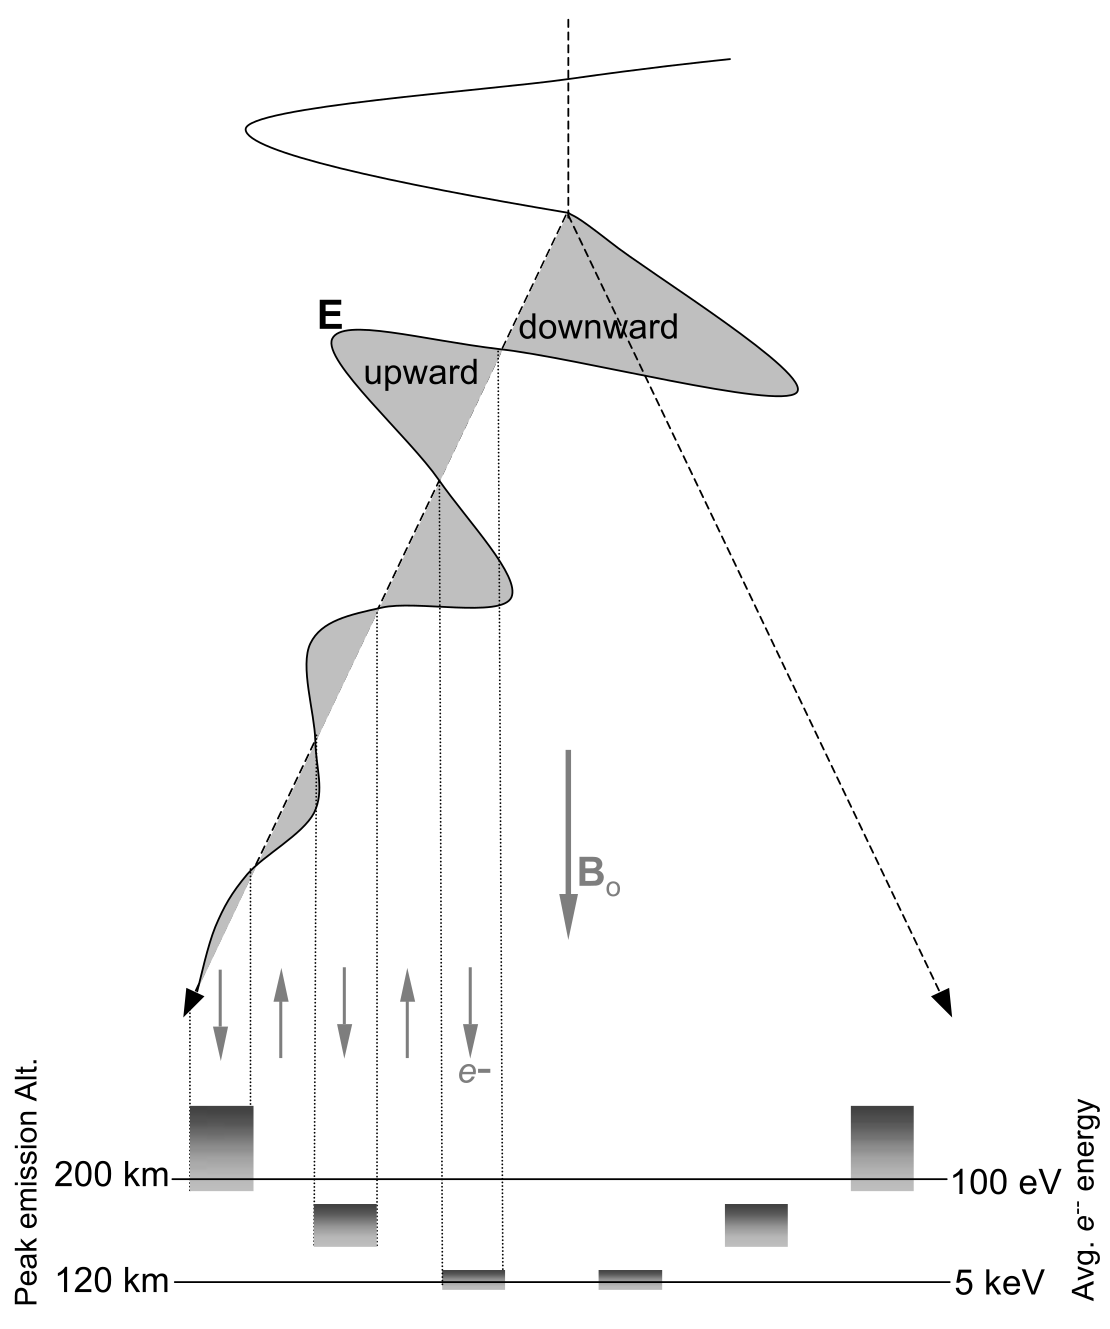
\includegraphics[width=0.9\linewidth]{gfx/alfven_cone}
	\caption{Alfvén wave acceleration cone structure with alternating up/down acceleration \citep{semeter2008}}\label{fig:alfvencone}
\end{figure}

%\subsection{Alfvén waves in the upper magnetosphere}
%Kinetic Alfvén waves (KAW) were first measured by the Polar satellite \citep{wygant2002} to have narrow widths of order 20~km.
%This is on the order of the ion-acoustic gyroradius, which facilitates KAW particle acceleration along $B_\parallel$.
%
%\citet{lysak1996} cited an Alfvén dispersion relation that treats the KAW-IAW-electrostatic regime as a continuüm throughout the DAW acceleration lifecycle.
%
%Alfvén wave-driven pulsating aurora has also been observed \citep{fukuda2016}.
Observational cadence with high-resolution electron spectrometers was typically of order of \unit[30..50]{ms} \citep{michell2016} on rockets and satellites such as MMS.
\citet{michell2016} motivated the new millisecond sampling electron spectrometer flown aboard the 2014 GREECE rocket by noting that auroral microstructure has sub-\unit[100]{m} widths and apparent $B_\perp$ velocities of up to \unit[20]{km/s}.
Nyquist theorem requires sampling at least as fast as $100/20000/2 = \unit[2.5]{ms}$.
Figure~\ref{fig:greece-precip} shows that \unit[1]{ms} is adequate for catching numerous DAW coming in rapid succession on this flight.
\begin{figure}
	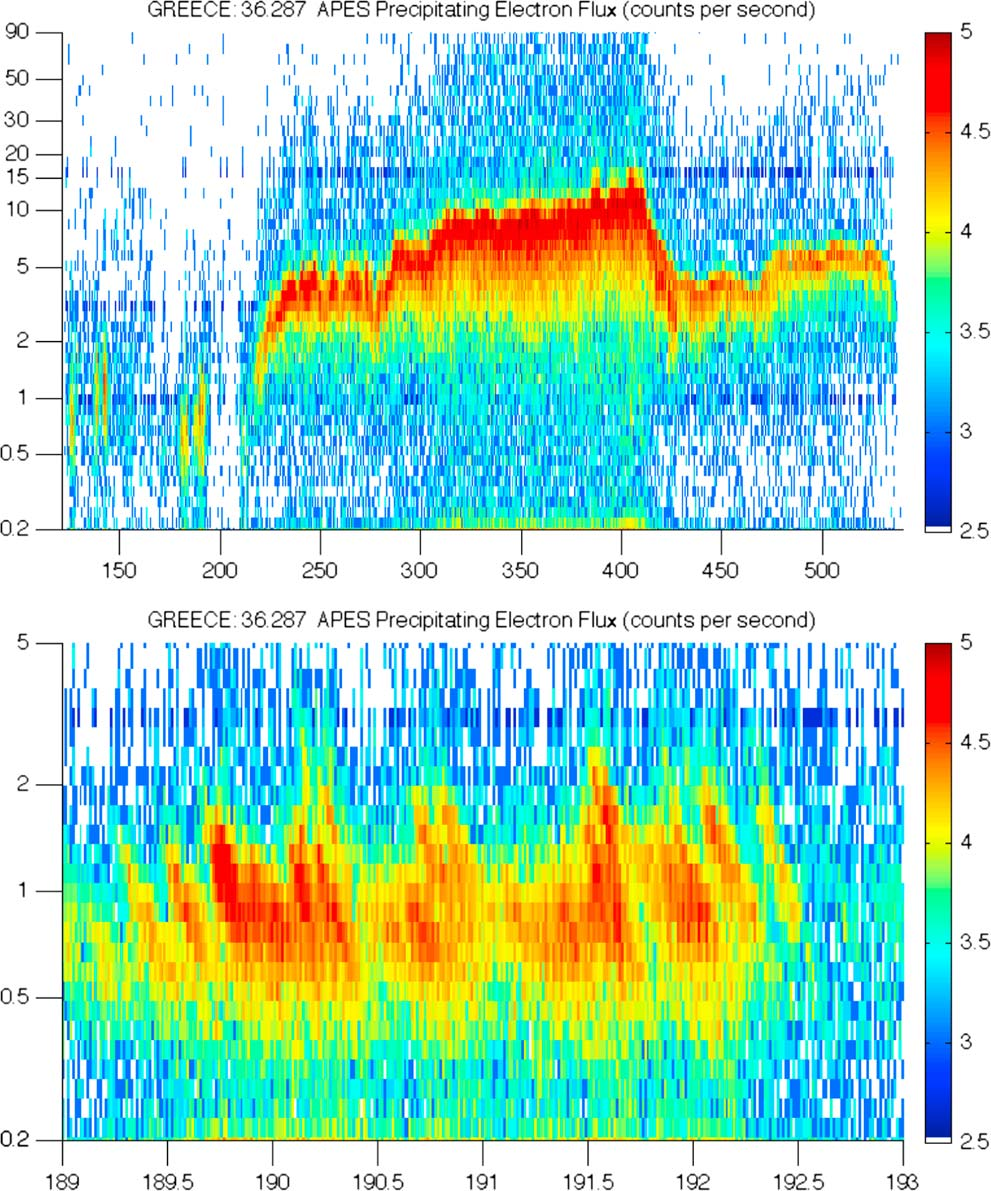
\includegraphics[width=\linewidth]{../gfx/greece-flux}
	\caption{Dispersive flux packets on GREECE rocket. \citep{michell2016}}
	\label{fig:greece-precip}
\end{figure}
The optical instrumentation described in chapter~\ref{chapter:inst} and the ISR described in chapter~\ref{chapter:fusion} are likewise of adequate sampling rate to resolve Alfvénic aurora.
A key distinction is that cameras can turn on and run indefinitely, thanks to the algorithm of chapter~\ref{chapter:discrim}, giving better chances for joint instrument observations.
Rockets and satellite provide invaluable \textit{in situ} measurements, but only for a single rapidly moving point (or cluster of points) in time.
Having rounded out the introductory theory necessary for the HiST system design, chapter~\ref{chapter:inst} describes the DMC and HiST systems, along with ISR and other instruments used in the joint ISR-optical analysis.
